Transient types represent a novel exchange of guarantees for performance;
 however, they suffer major limitations.
For one, the transient guarantees are so weak that types can mislead
 programmers trying to understand a faulty program.
Second, the transient type enforcement strategy adds overhead to all typed code;
 by contrast, natural types are only expensive when typed and untyped code interact.
To illustrate the differences on fully-typed programs,
 \figureref{fig:icfp-bars} compares the performance improvement
 in fully-typed (natural) Typed Racket code over untyped to the improvement in a
 transient Racket prototype.

\begin{figure}[h]
  % TODO log scale, add X for overhead, darker stripes (dude its fine)
  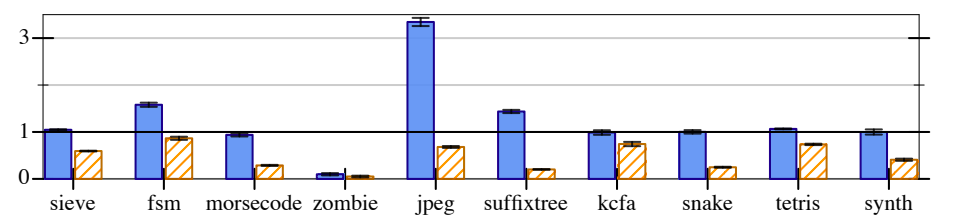
\includegraphics[width=0.8\columnwidth]{src/icfp-bars.png}
  \caption{Speedup factor of Typed Racket vs. untyped (solid bars) and a transient Racket vs. untyped (striped bars)~\cite{gf-icfp-2018}.
           Taller bars are better; bars below the 1x line indicate slowdowns.}
  \label{fig:icfp-bars}
\end{figure}

\noindent
The above brings us to the central question of my dissertation research:

\begin{quote}
  \emph{Does migratory typing benefit from a combination of \tdeep{} and \tshallow{} types?}
%% well ... we mean a particular combination with some angelic guidance from the programmer
\end{quote}

I plan to explore a combination of the natural and transient approaches to
 run-time type enforcement within one migratory typing system.
In the combined system, each component in a program shall be either:
 dynamically-typed,
 statically-typed with natural type enforcement,
 or statically-typed with transient type enforcement.
Both variants of static typing shall employ the same language of types and the
 same type checker.
Honest types must continue to be honest
 and lying types must continue to be type-sound
 in the weakened sense described in \sectionref{sec:done}.

Beyond the dominant question, two derivative questions must be addressed.
The first is \emph{how to combine}\/ honest and lying
 types in a way that preserves their respective guarantees.
The second is \emph{how to measure the performance benefit}\/ of the combination.
\Sectionref{sec:todo} outlines criteria and proposes solutions.

